% -*- latex -*-
%%%%%%%%%%%%%%%%%%%%%%%%%%%%%%%%%%%%%%%%%%%%%%%%%%%%%%%%%%%%%%%%
%%%%%%%%%%%%%%%%%%%%%%%%%%%%%%%%%%%%%%%%%%%%%%%%%%%%%%%%%%%%%%%%
%%%%
%%%% This text file is part of the source of 
%%%% `Introduction to High-Performance Scientific Computing'
%%%% by Victor Eijkhout, copyright 2012-6
%%%%
%%%% This book is distributed under a Creative Commons Attribution 3.0
%%%% Unported (CC BY 3.0) license and made possible by funding from
%%%% The Saylor Foundation \url{http://www.saylor.org}.
%%%%
%%%%
%%%%%%%%%%%%%%%%%%%%%%%%%%%%%%%%%%%%%%%%%%%%%%%%%%%%%%%%%%%%%%%%
%%%%%%%%%%%%%%%%%%%%%%%%%%%%%%%%%%%%%%%%%%%%%%%%%%%%%%%%%%%%%%%%

\index{sorting!bubblesort|see{bubblesort}}
\index{sorting!Quicksort|see{Quicksort}}
\index{sorting!Bitonic sort|see{Bitonic sort}}
\index{sorting!Samplesort|see{Samplesort}}

\label{sec:sorting}
\index{sorting|(}

Sorting is not a common operation in scientific computing: one expects
it to be more important in databases, whether these be financial or
biological (for instance in sequence alignment). However, it sometimes
comes up, for instance in \indexac{AMR} and other applications where
significant manipulations of data structures occurs.

In this section we will briefly look at some basic 
algorithms and how they can be done in parallel. For more details,
see~\cite{Kumar:parcomp-book} and the references therein.

\Level 0 {Brief introduction to sorting}

\Level 1 {Complexity}

There are many sorting algorithms. Traditionally, they have 
been distinguished by
their computational complexity, that is, given an array of $n$
elements, how many operations does it take to sort them, as a function
of~$n$. 

Theoretically one can show that a sorting algorithm has to have at
least complexity~$O(n\log n)$\footnote{One can consider a sorting
  algorithm as a decision tree: a first comparison is made, depending
  on it two other comparisons are made, et cetera. Thus, an actual
  sorting becomes a path through this decision tree. If every path has
  running time~$h$, the tree has $2^h$ nodes. Since a sequence of $n$
  elements can be ordered in $n!$ ways, the tree needs to have enough
  paths to accomodate all of these; in other words, $2^h\geq
  n!$. Using Stirling's formula, this means that $n\geq O(n\log
  n)$}. There are indeed several algorithms that are guaranteed to
attain this complexity, but a very popular algorithm, called
\indexterm{Quicksort} has only an `expected' complexity of~$O(n\log
n)$, and a worst case complexity of~$O(n^2)$. This behaviour results
from the fact that quicksort needs to choose `pivot elements' (we will
go into more detail below in section~\ref{sec:quicksort}), and if
these choices are consistently the worst possible, the optimal
complexity is not reached.

\begin{displayalgorithm}
  \While{the input array has length~$>1$}{
    Find a pivot element of intermediate size\;
    Split the array in two, based on the pivot\;
    Sort the two arrays.
  }
  \caption{The quicksort algorithm}
\end{displayalgorithm}

On the other hand, the very simple \indexterm{bubble sort} algorithm
always has the same complexity, since it has a static structure:

\begin{displayalgorithm}
  \For{$\mathit{pass}$ from $1$ to $n-1$}{
    \For{$e$ from 1 to $n-\mathit{pass}$}{
      \If{elements $e$ and $e+1$ are ordered the wrong way}{exchange
      them}
    }
  }
  \caption{The bubble sort algorithm}
\end{displayalgorithm}

It is easy to see that this algorithm has a complexity of~$O(n^2)$:
the inner loop does $t$ comparisons and up to $t$ exchanges. Summing
this from $1$ to $n-1$ gives approximately $n^2/2$ comparisons and
at most the same number of exchanges.

\Level 1 {Sorting networks}

Above we saw that some sorting algorithms operate independently of the
actual input data, and some make decisions based on that data.
The former class is sometimes
called \indextermbus{sorting}{network}. It can be considered
as custom hardware that implements just one algorithm. The 
basic hardware element is the \indexterm{compare-and-swap}
element, which has two inputs and two outputs. For two inputs $x,y$
the outputs are $\max(x,y)$ and $\min(x,y)$.

In figure~\ref{fig:bubble-pass} we show buble sort, built up
%
\begin{figure}[ht]
  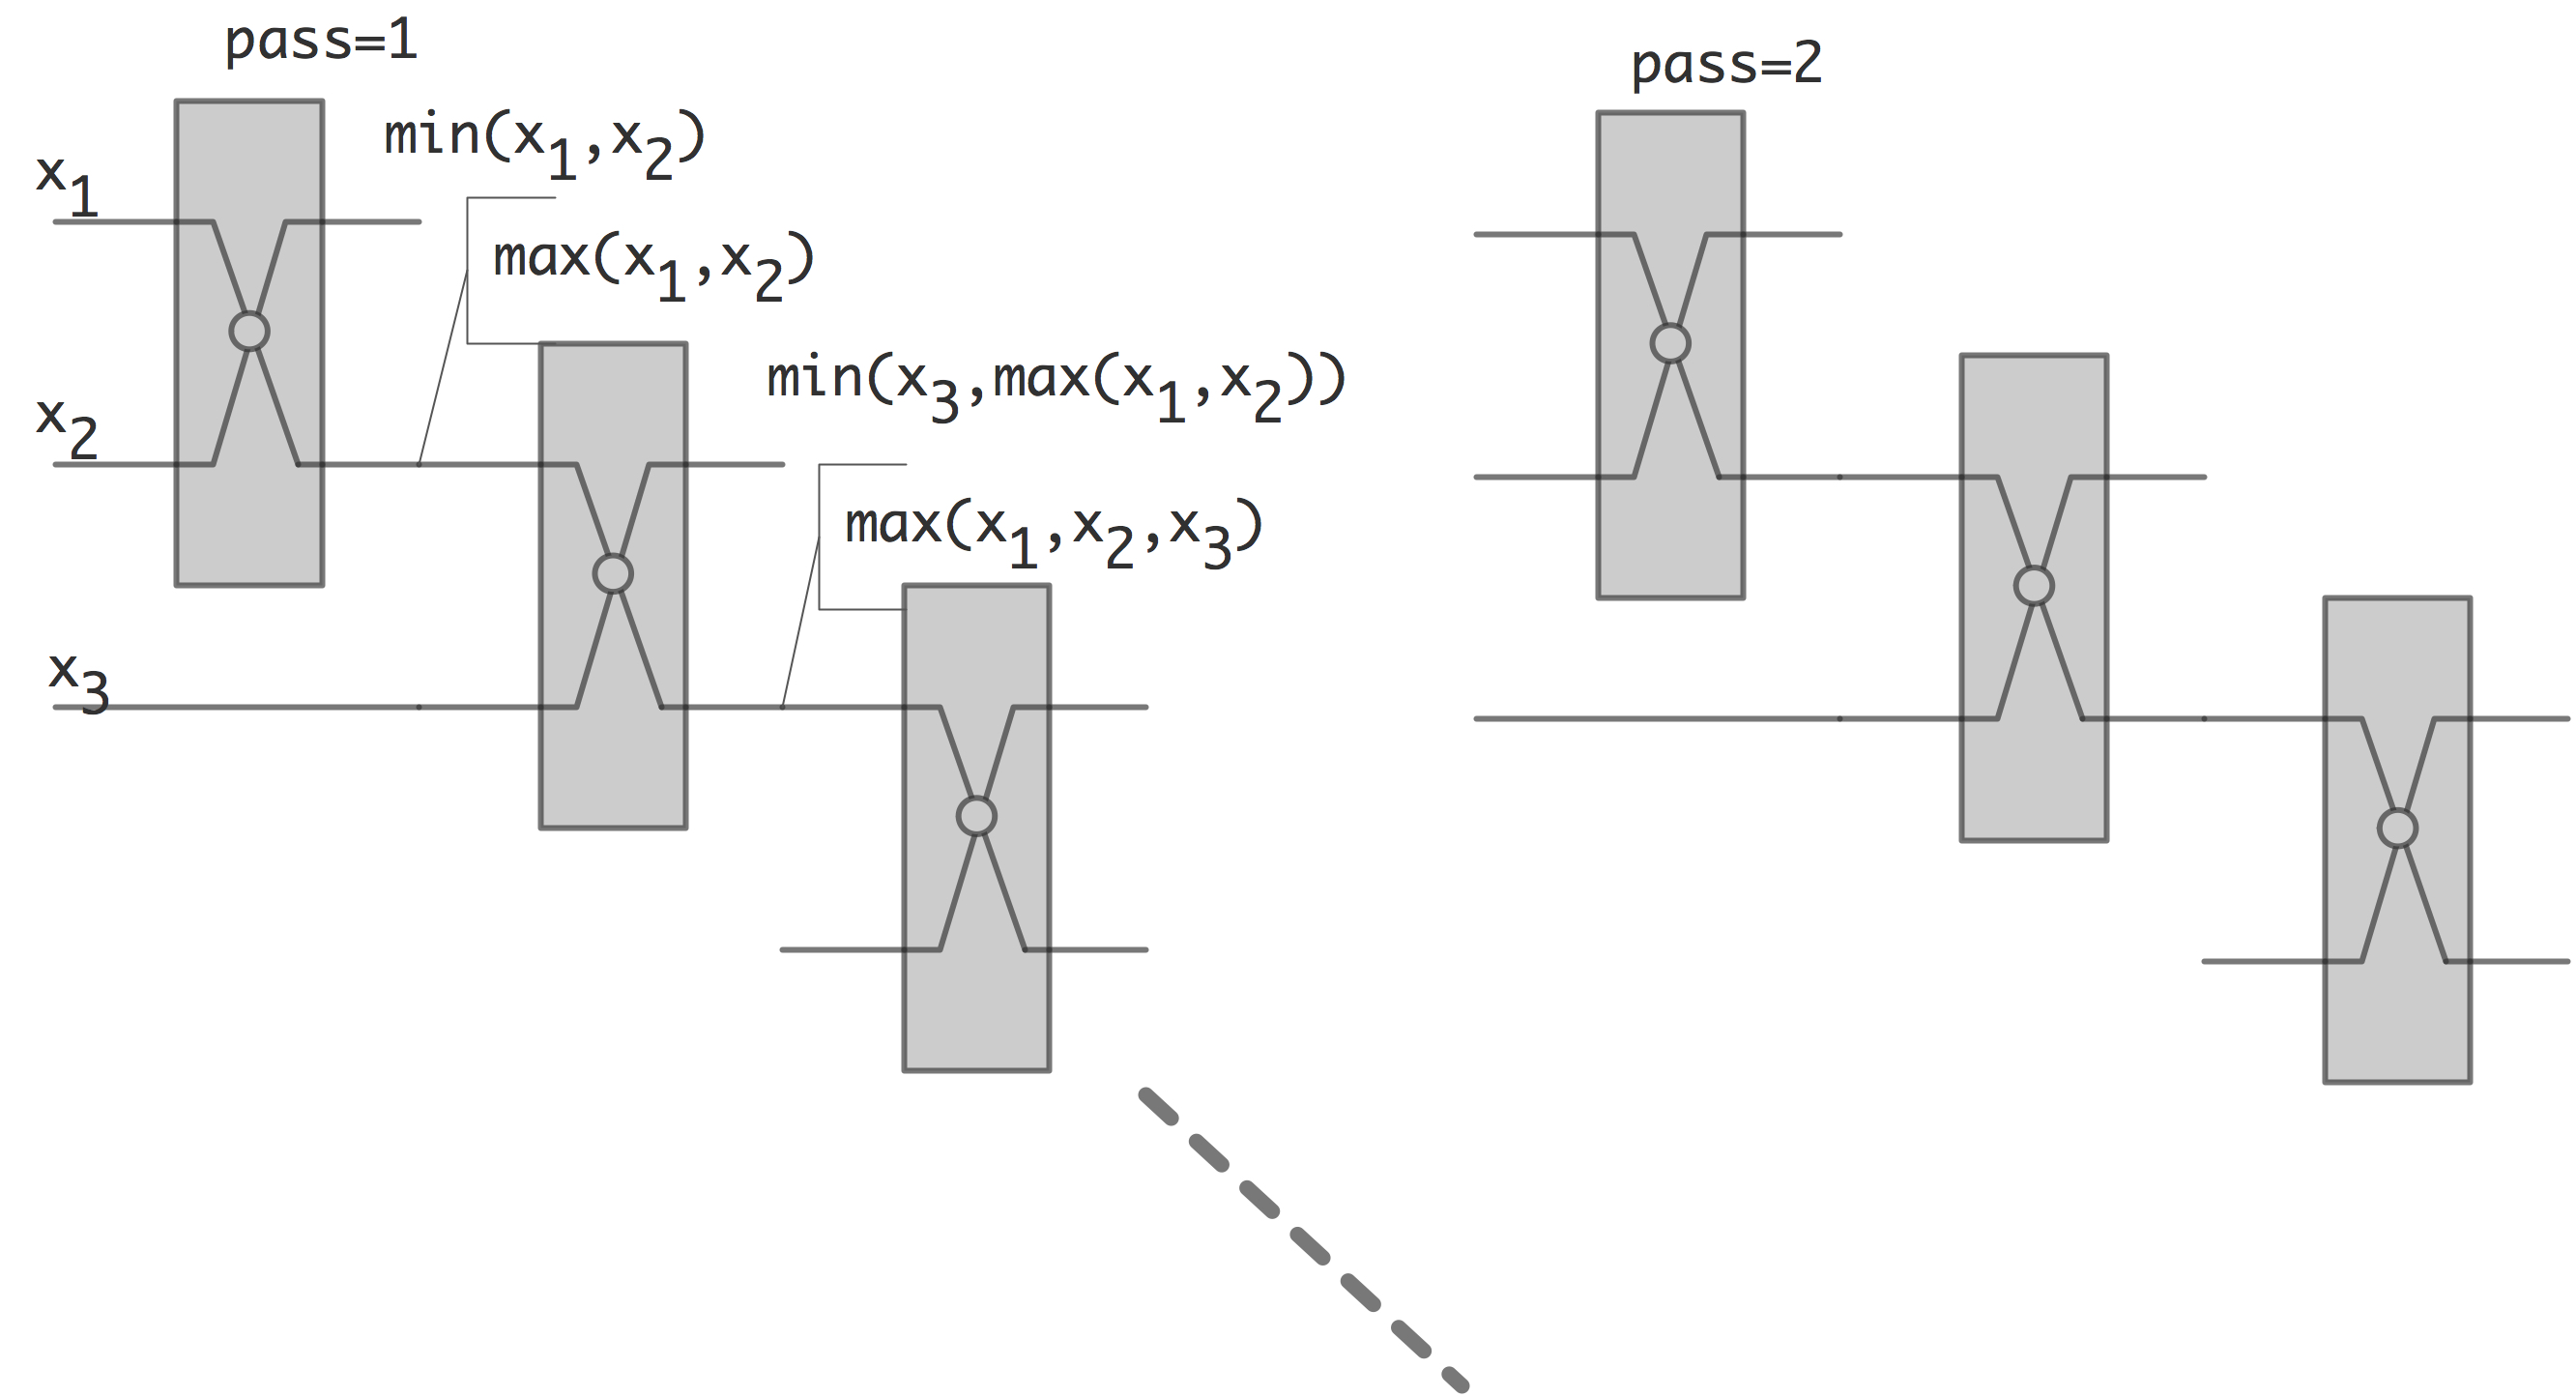
\includegraphics[scale=.13]{bubble-pass}
  \caption{Bubble sort as a sorting network}
  \label{fig:bubble-pass}
\end{figure}
%
out of compare and swap elements.

Below we will consider the \indexterm{Bitonic sort} algorithm
as a prime example of a sorting network.

\Level 1 {Parallel complexity}

Above we remarked that sorting sequentially takes at least $O(N\log N)$ time.
If we can have perfect speedup, using for simplicity $P=N$ processors,
we would have parallel time~$O(\log N)$. If the parallel time
is more than that, we define the \indexterm{sequential complexity}
as the total number of operations. For instance, below you will see
\indexterm{odd-even transposition sort},
also called \emph{swap sort}\index{swap sort|see{odd-even transposition
    sort}}
or \emph{exchange sort}\index{exchange sort|see{odd-even transposition
    sort}}.
This takes~$N$ parallel steps,
giving a sequential complexity of~$N^2$, and bitonic sort
which has a parallel time of~$(\log N)^2$ and a
sequential complexity of~$N(\log N)^2$.

\Level 0 {Odd-even transposition sort}
\index{odd-even transposition sort|(textbf}

Taking another look at figure~\ref{fig:bubble-pass}, you see that the
second pass
%
\begin{figure}[ht]
  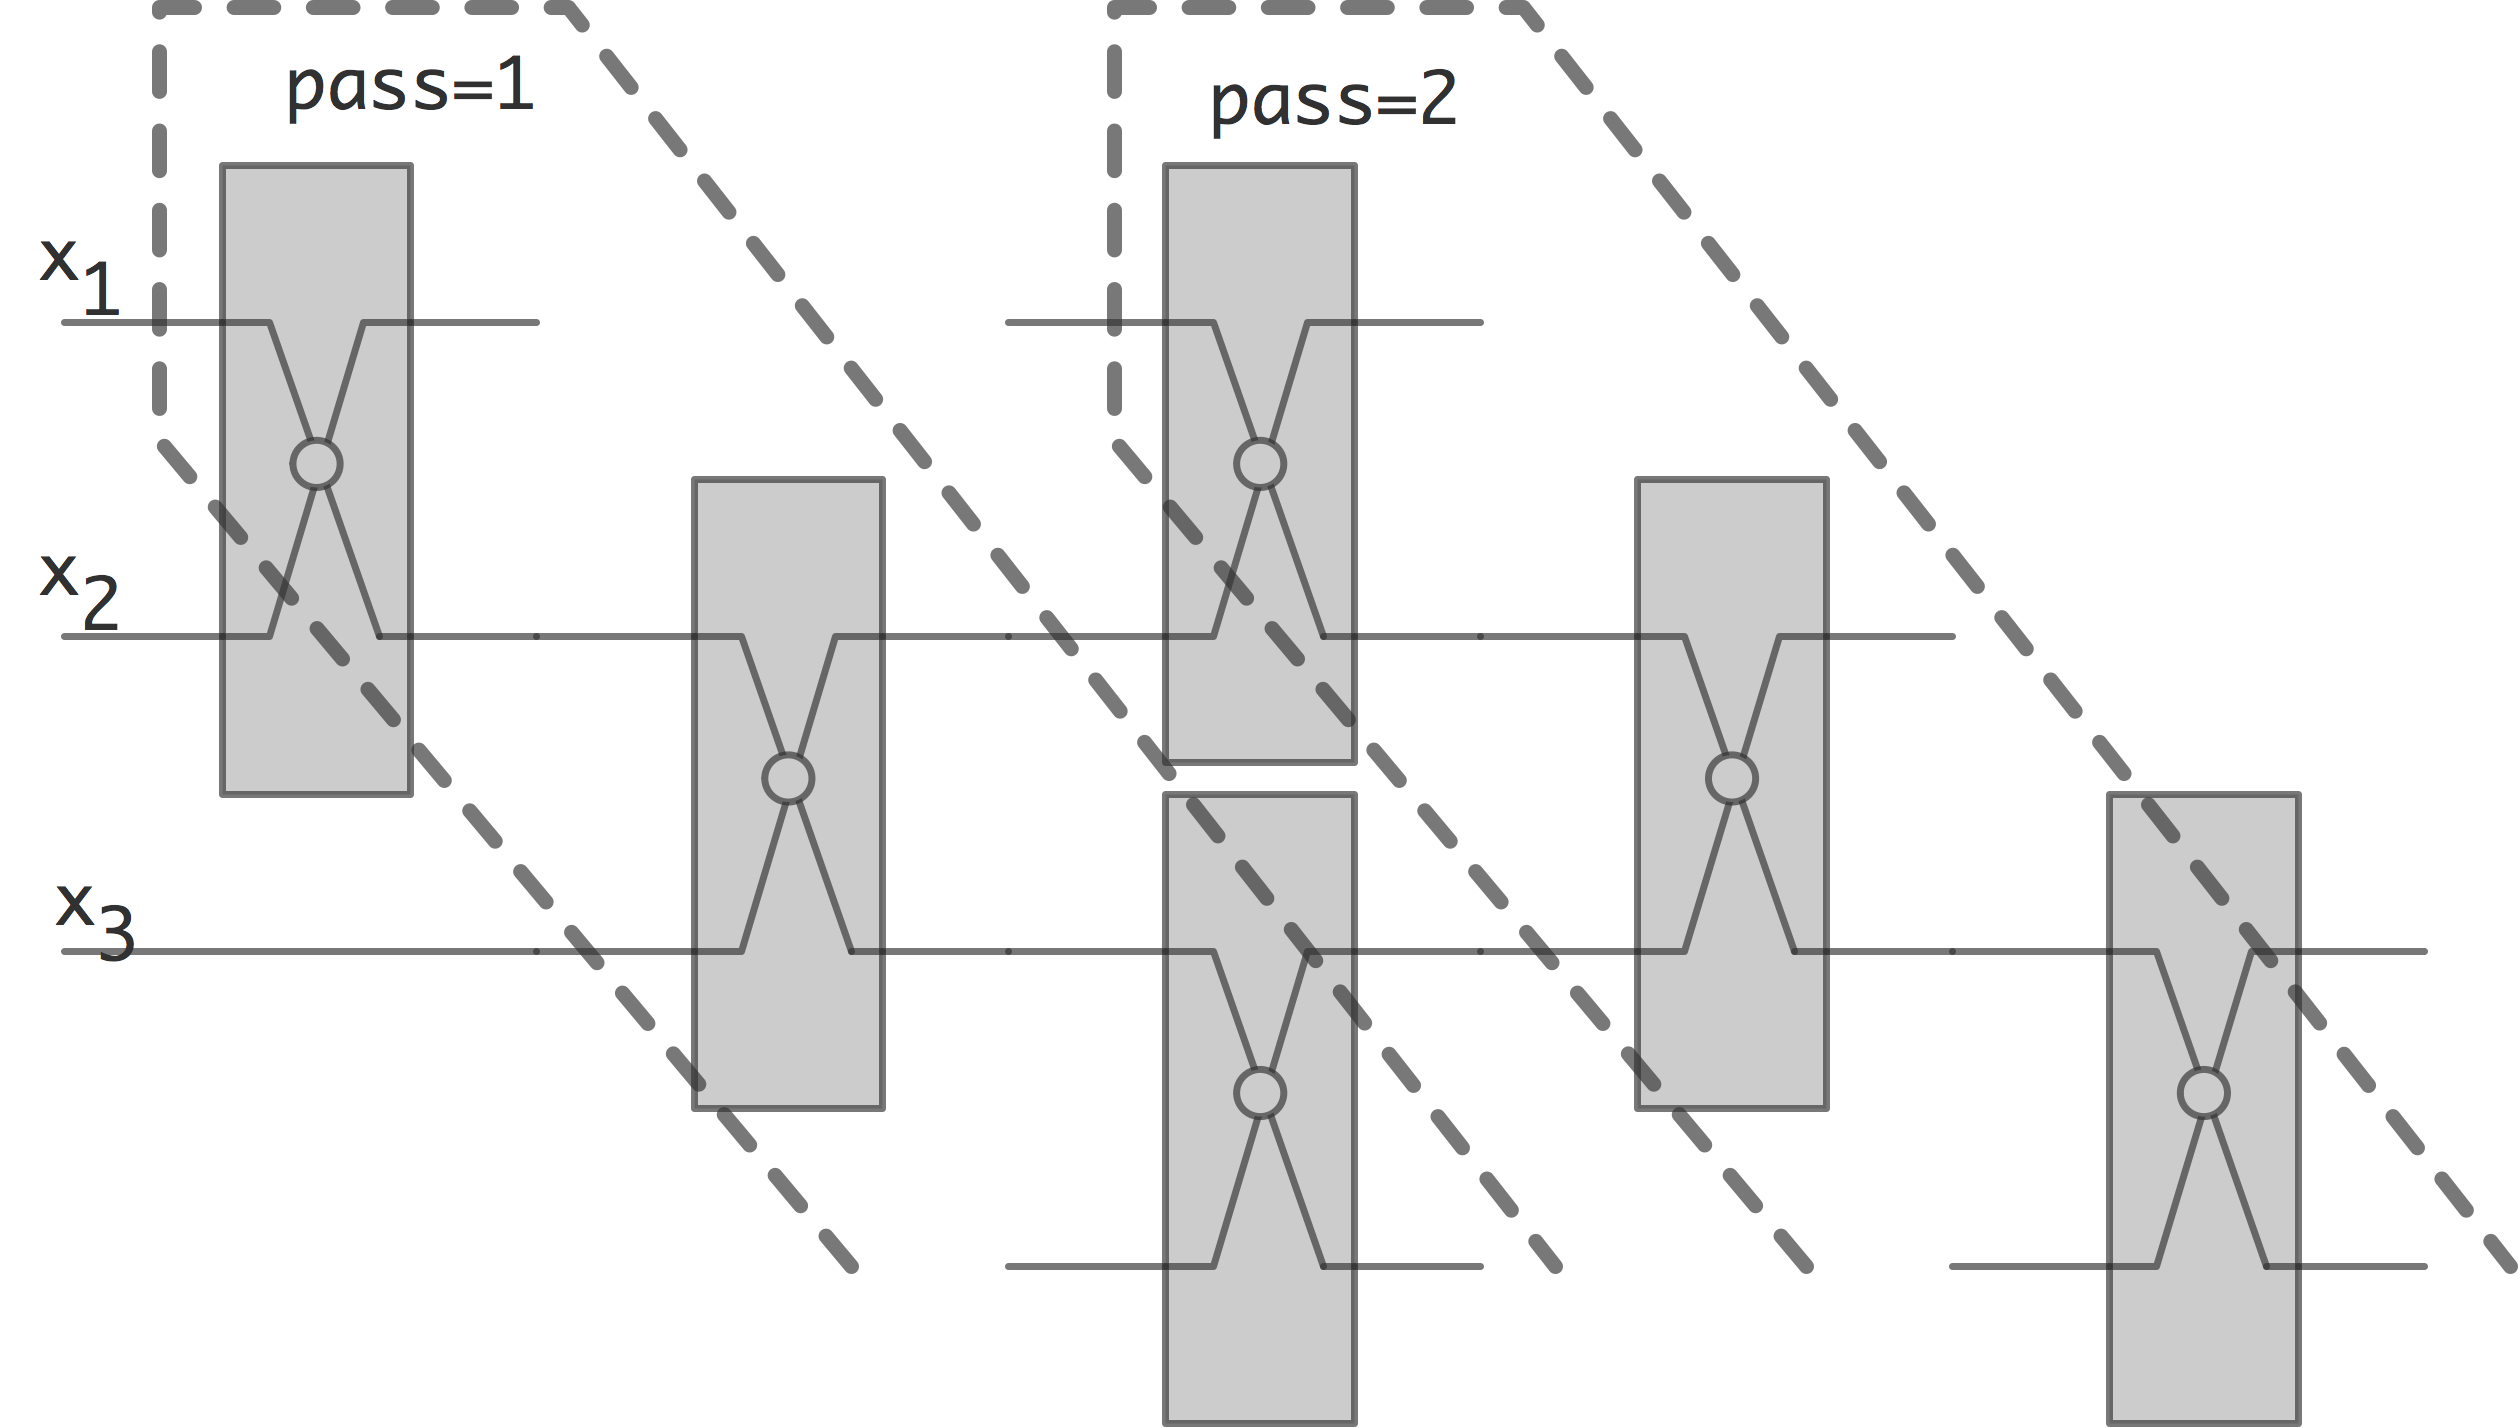
\includegraphics[scale=.12]{bubble-collapse}
  \caption{Overlapping passes in the bubble sort network}
  \label{fig:bubble-collapse}
\end{figure}
%
can actually be started long before the first pass is totally
finished. This is illustrated in figure~\ref{fig:bubble-collapse}.
If we now look at what happens at any given time, we easily derive the 
\emph{odd-even transposition sort} algorithm.

Odd-even transposition sort is a simple parallel sorting
algorithm, with as main virtue that it is easily implemented
on a linear area of processors. A~single step of the
algorithm consists of two substeps:
\begin{itemize}
\item Every even-numbered processor does a compare-and-swap
  with its right neighbour; then
\item Every odd-numbered processor does a compare-and-swap
  with its right neighbour.
\end{itemize}

\begin{theorem}
  After $N/$ steps, each consisting of the two substeps just given,
  a sequency is sorted.
\end{theorem}
\begin{proof}
  In each triplet $2i,2i+1,2i+2$, after an even and an odd step the
  largest element will be in rightmost position. Proceed by induction.
\end{proof}

With a parallel time of $N$, this gives a sequential complexity~$N^2$
compare-and-swap operations.

\begin{exercise}
  \label{ex:swapsort}
  Discuss speedup and efficiency of swap sort, where we sort $N$
  numbers of $P$ processors; for simplicity we set $N=P$ so that
  each processor contains a single number. Express execution time
  in \indexterm{compare-and-swap} operations.
  \begin{enumerate}
  \item How many compare-and-swap operations does the parallel code
    take in total?
  \item How many sequential steps does the algorithm take? What are
    $T_1$, $T_p$, $T_\infty$, $S_p$, $E_p$ for sorting $N$ numbers?
    What is the average amount of parallelism?
  \item Swap sort can be considered a parallel implementation of
    bubble sort. Now let $T_1$ refer to the execution time of
    (sequential) bubble sort. How does this change $S_p$ and~$E_p$?
  \end{enumerate}
\end{exercise}

\index{odd-even transposition sort|)textbf}

\Level 0 {Quicksort}
\label{sec:quicksort}
\index{Quicksort|(}

Quicksort is a recursive algorithm, that, unlike bubble sort, is not
deterministic. It is a two step procedure, based on a reordering of
the sequence\footnote{The name is explained by its origin with the
  Dutch computer scientist Edsger Dijkstra; see
  \url{http://en.wikipedia.org/wiki/Dutch_national_flag_problem}.}:

\begin{displayalgorithm}
  \TitleOfAlgo{Dutch National Flag ordering of an array}
  \Input{An array of elements, and a `pivot' value}
  \Output{The input array with elements ordered as red-white-blue,
    where red elements are larger than the pivot, white elements are
    equal to the pivot, and blue elements are less than the pivot}
\end{displayalgorithm}

We state without proof that this can be done in $O(n)$ operations.
With this, quicksort becomes:

\begin{displayalgorithm}
  \TitleOfAlgo{Quicksort}
  \Input{An array of elements}
  \Output{The input array, sorted}
  \While{The array is longer than one element}{
    pick an arbitrary value as pivot \;
    apply the Dutch National Flag reordering to this array \;
    Quicksort( the blue elements ) \; Quicksort( the red elements ) \;
  }
\end{displayalgorithm}

The indeterminacy of this algorithm, and the variance in its
complexity, stems from the pivot choice. In the worst case, the pivot
is always the (unique) smallest element of the array. There will then
be no blue elements, the only white element is the pivot, and the
recursive call will be on the array of $n-1$ red elements. It is easy
to see that the running time will then be~$O(n^2)$. On the other hand,
if the pivot is always (close to) the median, that is, the element
that is intermediate in size, then the recursive calls will have an
about equal running time, and we get a recursive formula for the
running time:
\[ T_n = 2T_{n/2} + O(n) \]
which  is (again without proof) $O(n\log n)$.

We will now consider parallel implementations of quicksort.

\Level 1 {Quicksort in shared memory}

A simple parallelization of the quicksort algorithm can be achieved by
executing the two recursive calls in parallel. This is easiest
realized with a shared memory model, and threads
(section~\ref{sec:threads}) for the recursive calls. However, this
implementation is not efficient. 

On an array of length~$n$, and with perfect pivot choice, there will
be $n$~threads active in the final stage of the algorithm. Optimally,
we would want a parallel algorithm to run in $O(\log n)$ time, but
here the time is dominated by the initial reordering of the array by
the first thread.

\begin{exercise}
  Make this argument precise. What is the total running time, the
  speedup, and the efficiency of parallelizing the quicksort algorithm
  this way?
\end{exercise}

Is there a way to make splitting the array more efficient?
As it turns out, yes, and the key is to use a parallel \indexterm{prefix
operation}; see appendix~\ref{app:prefix}. If the array of values
is $x_1,\ldots,x_n$, we use a parallel prefix to compute
how many elements are less than the pivot~$\pi$:
\[ X_i=\#\{ x_j\colon j<i\wedge x_j<\pi \}. \]
With this, if a processor looks at~$x_i$, and $x_i$~is less
than the pivot, it needs to be moved to location~$X_i+1$
in the array where elements are split according to the pivot.
%
Similarly, one would could how many elements there are over the pivot,
and move those accordingly.

This shows that each pivoting step can be done in $O(\log n)$ time,
and since there $\log n$ steps to the sorting algorithm, the
total algorithm runs in $O((\log n)^2)$ time.

\Level 1 {Quicksort on a hypercube}

As was apparent from the previous section, for an efficient
parallelization of the quicksort algorithm, we need to make the Dutch
National Flag reordering parallel too. Let us then assume that the
array has been partitioned over the $p$ processors of a hypercube of
dimension~$d$ (meaning that $p=2^d$).

In the first step of the parallel algorithm, we choose a pivot, and
broadcast it to all processors. All processors will then apply the
reordering independently on their local data. 

In order to bring together the red and blue elements in this first
level, every processor is now paired up with one that has a binary
address that is the same in every bit but the most significant one. In
each pair, the blue elements are sent to the processor that has a
1~value in that bit; the red elements go to the processor that has a
0~value in that bit.

After this exchange (which is local, and therefore fully parallel),
the processors with an address $1xxxxx$ have all the red elements, and
the processors with an address $0xxxxx$ have all the blue
elements. The previous steps can now be repeated on the subcubes.

This algorithm keeps all processors working in every step; however, it
is susceptible to load imbalance if the chosen pivots are far from the
median. Moreover, this load imbalance is not lessened during the sort
process.

\Level 1 {Quicksort on a general parallel processor}

Quicksort can also be done on any parallel machine that has a linear
ordering of the processors. We assume at first that every processor
holds exactly one array element, and, because of the flag reordering,
sorting will always involve a consecutive set of processors.

Parallel quicksort of an array (or subarray in a recursive call)
starts by constructing a binary tree on the processors storing the
array. A~pivot value is chosen and broadcast through the tree. The
tree structure is then used to count on each processor how many
elements in the left and right subtree are less than, equal to, or
more than the pivot value. 

With this information, the root processor can compute where the
red/white/blue regions are going to be stored. This information is
sent down the tree, and every subtree computes the target locations
for the elements in its subtree.

If we ignore network contention, the reordering can now be done in
unit time, since each processor sends at most one element. This means
that each stage only takes time in summing the number of blue and red
elements in the subtrees, which is $O(\log n)$ on the top level,
$O(\log n/2)$~on the next, et cetera. This makes for almost perfect
speedup.

\index{Quicksort|)}

\Level 0 {Samplesort}
\label{sec:samplesort}
\index{Samplesort|(textbf}

You saw in \indexterm{Quicksort} (section~\ref{sec:quicksort}) that
it is possible to use probabilistic elements in a sorting
algorithm. We can extend the idea of picking a single pivot, as in
Quicksort, to that of picking as many pivots as there are processors.
Instead of a \indexterm{bisection} of the elements, this divides the
elements into as many `buckets' as there are processors. Each
processor then sorts its elements fully in parallel.

\begin{displayalgorithm}
  \Input{$p$: the number of processors, $N$: the numbers of elements to
    sort; $\{x_i\}_{i<N}$ the elements to sort}
  Let $x_0=b_0<b_1<\cdots<b_{p-1}<b_p=x_N$ (where $x_N>x_{N-1}$ arbitrary)\;
  \For { $i=0,\ldots,p-1$ } { Let $s_i=[b_i,\ldots b_{i+1}-1]$ }
  \For { $i=0,\ldots,p-1$ } { Assign the elements in $s_i$ to
    processor~$i$ }
  \For { $i=0,\ldots,p-1$ in parallel } { Let processor~$i$ sort its
    elements }
  \caption{The Samplesort algorithm}
\end{displayalgorithm}

Clearly this algorithm can have severe \indextermbus{load}{imbalance}
if the buckets are not chosen carefully. Randomly picking $p$ elements is
probably not good enough; instead, some form of \indexterm{sampling}
of the elements is needed. Correspondingly, this algorithm is known as
\textbf{Samplesort}.

While the sorting of the buckets, once assigned, is fully parallel,
this algorithm still has some problems regarding parallelism.
First of all, the sampling is a sequential bottleneck for the algorithm.
Also, the step where buckets are assigned to processors is essentially
an \indexterm{all-to-all} operation, which becomes a network
bottleneck.
Note that in Quicksort on a hypercube there was never any
\indexterm{contention} for the wires.

\index{Samplesort|)}

\Level 0 {Bitonic sort}
\label{app:bitonicsort}
\index{bitonic sort|(textbf}

To motivate bitonic sorting,
suppose a sequence $x=\langle x_0,\ldots,x_n-1\rangle$
consists of an ascending
followed by a descending part.
\begin{figure}[h]
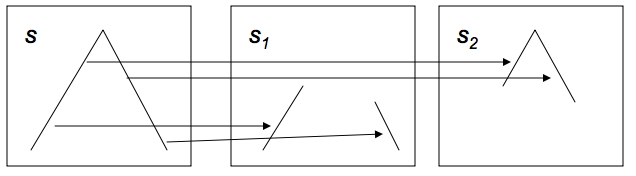
\includegraphics[scale=.5]{bitonic1}
\caption{Illustration of a splitting a bitonic sequence}
\end{figure}
Now split this sequence into two subsequences of equal length
defined by:
\begin{equation}
\begin{array}{cc}
s_1 = \langle \min\{x_0,x_{n/2}\},\ldots \min\{ x_{n/2-1},x_{n-1}\}\\
s_2 = \langle \max\{x_0,x_{n/2}\},\ldots \max\{ x_{n/2-1},x_{n-1}\}\\
\end{array}
\label{eq:bitonic-split}
\end{equation}
From the picture it is easy to see that $s_1,s_2$ are again 
sequences with an ascending and descending part. Moreover,
all the elements in $s_1$ are less than all the elements in~$s_2$.

We call \eqref{eq:bitonic-split} an ascending bitonic sorter, sinc the
second subsequence contains elements larger than in the
first. Likewise we can construct a descending sorter by reversing the
roles of maximum and minimum.

It's not hard to imagine that this is a step in a sorting algorithm:
starting out with a sequence on this form, recursive application 
of formula~\eqref{eq:bitonic-split} gives a sorted sequence.
\begin{figure}[h]
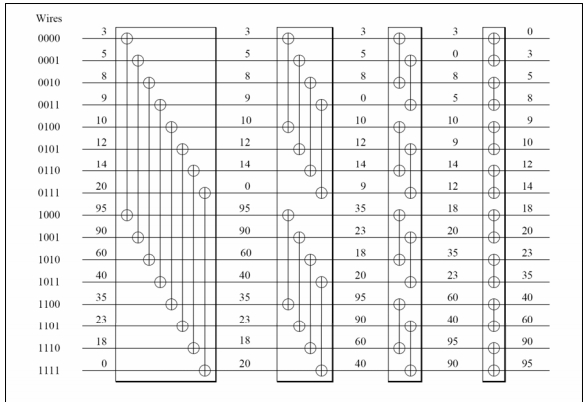
\includegraphics[scale=.5]{bitonic2}
\caption{Illustration of a  bitonic network that sorts a bitonic sequence of length~16}
\label{fig:bitonic8421}
\end{figure}
Figure~\ref{fig:bitonic8421} shows how 4 bitonic sorters, over
distances 8,4,2,1 respectively, will sort a sequence of length~16.

The actual definition of a \indexterm{bitonic sequence} is slightly more
complicated. A~sequence is bitonic if it conists of an ascending part followed 
by a descending part, or is a cyclic permutation of such a sequence.
\begin{exercise}
Prove that splitting a bitonic sequence according to
formula~\eqref{eq:bitonic-split} gives two bitonic sequences.
\end{exercise}

So the question is how to get a bitonic sequence. The answer is to
use larger and larger bitonic networks.
\begin{itemize}
\item A bitonic sort of two elements gives you a sorted sequence.
\item If you have two sequences of length two, one sorted up, the
  other sorted down, that is a bitonic sequence.
\item So this sequence of length four can be sorted in two bitonic steps.
\item And two sorted sequences of length four form a bitonic sequence of length;
\item which can be sorted in three bitonic steps; et cetera.
\end{itemize}
\begin{figure}[ht]
  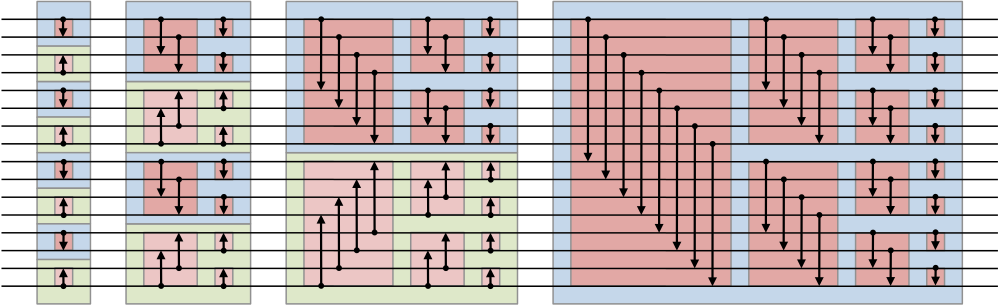
\includegraphics[scale=.4]{full-bitonic}
  \caption{Full bitonic sort for 16 elements}
  \label{fig:full-bitonic}
\end{figure}
From this description you see that you $\log_2N$ stages to sort $N$
elements, where the $i$-th stage is of length~$\log_2i$. This makes
the total \indextermsub{sequential complexity of}{bitonic sort}~$(\log_2N)^2$.

The sequence of operations in figure~\ref{fig:full-bitonic}
is called a \indextermbus{sorting}{network}, built up out of simple 
\indexterm{compare-and-swap} elements. There is no dependence 
on the value of the data elements, as is the case with quicksort.

\index{bitonic sort|)}

\index{sorting|)}

